% ============================
\renewcommand{\chaptername}{Errata}
\chapter{Les exceptions}
\label{chap:exceptions}
% ============================

\begin{Exergue}
	\og{}Attrapez-les tous, sans exception !\fg{}
\end{Exergue}

\minitoc

\section{Motivation}
Un programme ne tourne pas dans un monde idéal.

Il doit pouvoir \emph{résister aux défaillances} de l'environnement, telles que
  \begin{itemize}
  \item On tente d'ouvrir un fichier qui n'existe pas
  \item L'utilisateur entre des données incorrectes
  \item Une connexion à un site web ne se fait pas
  \item etc.
  \end{itemize}

  Tous ces évènements \emph{exceptionnels} viennent perturber le fonctionnement de votre programme, et doivent être gérés. Le langage Java offre un mécanisme, celui des exceptions.

À titre d'exemple, considérons le programme suivant

\begin{java}
import java.util.Scanner;
public class Affiche {
  /**
   * Affiche un nombre entier lu au clavier.
   * @param args non utilisé
   */
  public static void main(String[] args) {
      Scanner clavier = new Scanner(System.in);
      int nb;
 
      nb = clavier.nextInt();
      System.out.println(nb);
  }
}
\end{java}

Que se passe-t-il lorsque l'utilisateur entre une lettre, ou un nombre décimal ?

\begin{center}
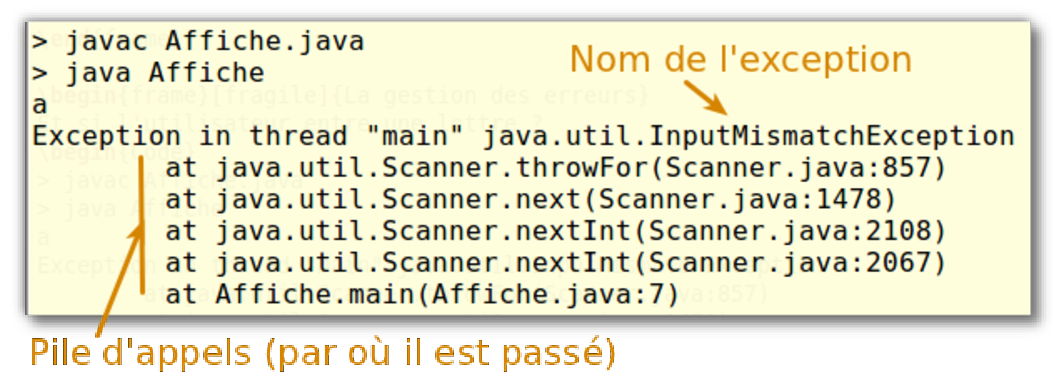
\includegraphics[scale=0.65]{images/exception-InputMismatchException.pdf}
\end{center}

On constate qu'une Exception a été levée (ou \og lancée\fg), ce qui résulte en l'arrêt prématuré du programme.

%\begin{Code}
%> javac Affiche.java
%> java Affiche
%a
%Exception in thread "main" java.util.InputMismatchException
%	at java.util.Scanner.throwFor(Scanner.java:857)
%	at java.util.Scanner.next(Scanner.java:1478)
%	at java.util.Scanner.nextInt(Scanner.java:2108)
%	at java.util.Scanner.nextInt(Scanner.java:2067)
%	at Affiche.main(Affiche.java:7)
%\end{Code}

\section{L'instruction \pc{try-catch}}
On l'a vu, une Exception peut arrêter l'exécution du programme. Cependant, le mécanisme autorise aussi d'intercepter (ou \og attraper\fg) les Exceptions, afin de traiter l'erreur de façon transparente pour l'utilisateur. On utilise à cet effet une instruction \pc{try-catch}, constituée de deux blocs de code :
\begin{itemize}
\item \pc{try} : contient les instructions qui \emph{peuvent mal se passer}
\item \pc{catch} : contient le code qui est \emph{en charge} de gérer le problème
\end{itemize}

Quand une exception est levée dans un \pc{try}
\begin{itemize}
\item Le code du \pc{try} est interrompu
\item Le code du \pc{catch} est exécuté
\item L'exécution reprend après le bloc \pc{try-catch}
\end{itemize}

À titre d'exemple, on peut ainsi intercepter les exceptions levées par \pc{nextInt()} comme ceci :
\begin{java}
import java.util.Scanner;
public class Affiche {
  /**
   * Affiche l'entier lu au clavier, ou un message si ce n'est pas un entier.
   * @param args inutilisé.
   */
  public static void main(String[] args) {
      Scanner clavier = new Scanner(System.in);
      int nb;
      try { 
        nb = clavier.nextInt();
        System.out.println(nb);
      }
      catch(Exception e) { 
        System.out.println("Ce n'est pas un entier!");
      }
  }
}
\end{java}

Afin d'être plus spécifique, on peut nommer dans le \pc{catch} l'exception précise à intercepter, par exemple \pc{InputMismatchException}.


\section{L'instruction \pc{throw}}
Imaginons la situation où un programme doit demander un \emph{entier positif} à l'utilisateur.
Si le programme ne vérifie pas immédiatement que le nombre donné est entier et positif, il s'expose à des problèmes tels que plantages, résultats erronés, perte ou corruption de données, etc.
avec la condition aggravante que le problème pourrait ne se signaler que plus loin dans le code, et plus tard dans le temps, rendant le déboguage plus difficile.
Cette constatation est à la base du mantra \og Fail early, fail loudly.\fg.

Cas pratique : vérifier les \emph{arguments} reçus.
Si un paramètre est supposé être un entier positif, une saine gestion consiste à vérifier que c'est le cas et à lever une exception sinon.

\begin{java}
  /**
   * Calcule la racine carrée d'un nombre.
   * @param nb le nombre dont on veut la racine carée.
   * @return la racine carrée de <code>nb<\code>.
   * @throws IllegalArgumentException si <code>nb</code> est négatif.
   */
  public static double racineCarrée(double nb) {
    if (nb<0) {
      throw new IllegalArgumentException("nb doit être positif!");
    }
    // Traitement normal. On est sûr que le paramètre est OK.
  }
\end{java}


\begin{java}
  try {
    System.out.println( racineCarrée( val ) );
  } catch (Exception ex) {
    System.out.println( "Calcul impossible !" );
  }
\end{java}

Comme annoncé précédemment, on peut aussi préciser qu'on n'intercepte \emph{que} les \pc{IllegalArgumentException}
\begin{java}
  try {
    System.out.println( racineCarrée( val ) );
  } catch (IllegalArgumentException ex) {
    System.out.println( "Calcul impossible !" );
  }
\end{java}



% %%% Local Variables:
% %%% TeX-master: "../dev1-dev-syllabus-master"
% %%% End:
